\documentclass[tikz,border=7pt]{standalone}
\usepackage{palatino}
\usepackage{amsmath}
\usepackage[none]{hyphenat}
\usepackage{xcolor}
\usetikzlibrary{arrows.meta,calc}

\definecolor{mapink}{HTML}{20252B}
\definecolor{mapgray}{HTML}{707780}
\definecolor{mapline}{HTML}{9199A1}
\definecolor{mapblue}{HTML}{0072B2}
\definecolor{mapbluefill}{HTML}{EAF3FA}
\definecolor{mapgreen}{HTML}{18857A}
\definecolor{mapgreenfill}{HTML}{E9F4F1}

\begin{document}
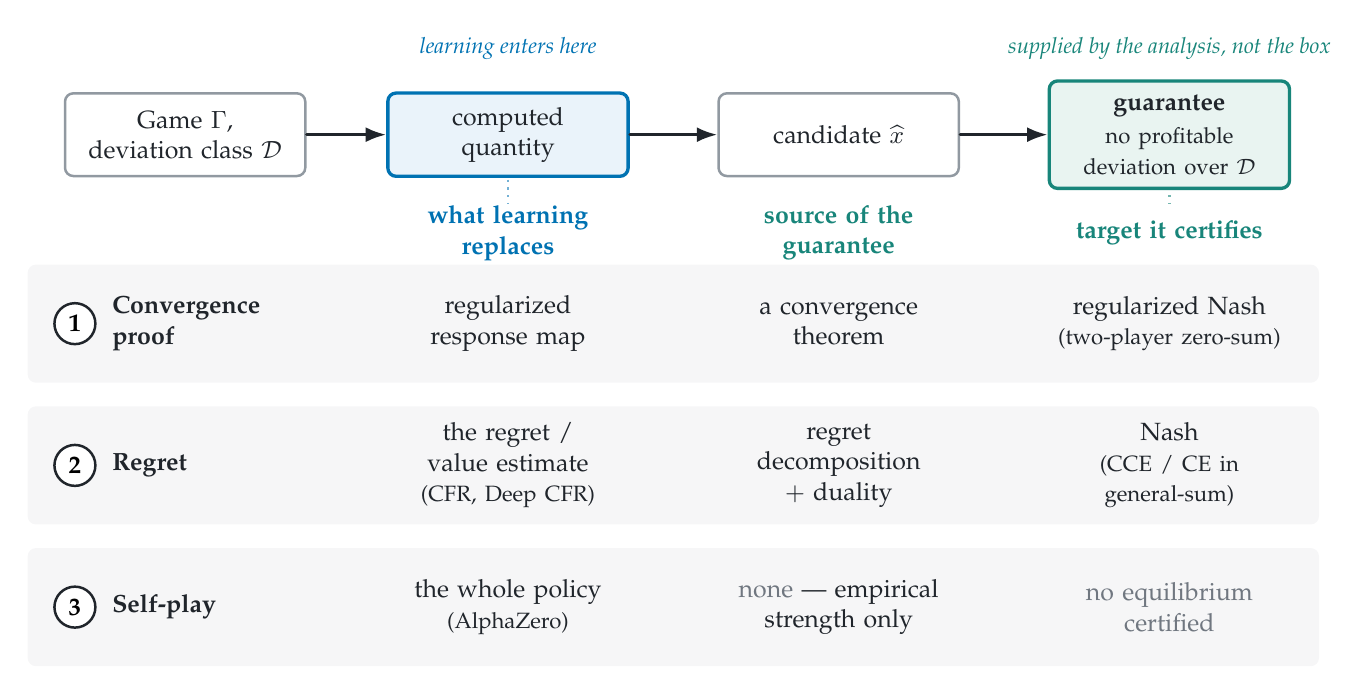
\begin{tikzpicture}[
  font=\rmfamily,
  pipe/.style={
    draw=mapline, fill=white, text=mapink, line width=0.9pt,
    rounded corners=3pt, align=center, font=\rmfamily\small,
    text width=2.7cm, minimum width=3.0cm, minimum height=1.05cm, inner sep=5pt
  },
  learnbox/.style={
    draw=mapblue, fill=mapbluefill, text=mapink, line width=1.2pt,
    rounded corners=3pt, align=center, font=\rmfamily\small,
    text width=2.7cm, minimum width=3.0cm, minimum height=1.05cm, inner sep=5pt
  },
  guarbox/.style={
    draw=mapgreen, fill=mapgreenfill, text=mapink, line width=1.2pt,
    rounded corners=3pt, align=center, font=\rmfamily\small,
    text width=2.7cm, minimum width=3.0cm, minimum height=1.05cm, inner sep=5pt
  },
  flow/.style={draw=mapink, line width=1.1pt, -{Latex[length=2.6mm,width=1.9mm]}, line cap=round},
  num/.style={circle, draw=mapink, fill=white, line width=0.9pt, minimum size=0.52cm, inner sep=0pt, font=\rmfamily\bfseries\small},
  cellA/.style={align=center, text width=3.0cm, font=\rmfamily\small, text=mapink},
  cellB/.style={align=center, text width=3.0cm, font=\rmfamily\small, text=mapink},
  cellC/.style={align=center, text width=3.3cm, font=\rmfamily\small, text=mapink},
]

% ---- pipeline coordinates ----
\def\yP{3.35}
\coordinate (cP1) at (-6.5,\yP);
\coordinate (cP2) at (-2.4,\yP);
\coordinate (cP3) at ( 1.8,\yP);
\coordinate (cP4) at ( 6.0,\yP);

% column x-centers for the lane block
\def\xA{-2.4} % what learning replaces  (under P2)
\def\xB{ 1.8} % source of the guarantee (under P3)
\def\xC{ 6.0} % target it certifies     (under P4)

% short connectors tying highlighted boxes to their columns
\draw[mapblue!55,  line width=0.8pt, dotted] (\xA,2.78) -- (\xA,2.48);
\draw[mapgreen!60, line width=0.8pt, dotted] (\xC,2.78) -- (\xC,2.48);

% lane backgrounds (behind)
\foreach \y in {0.95,-0.85,-2.65}{
  \fill[mapink!4, rounded corners=3pt] (-8.5,\y-0.75) rectangle (7.9,\y+0.75);
}

% ---- pipeline row ----
\node[pipe]     (P1) at (cP1) {Game $\Gamma$,\\ deviation class $\mathcal{D}$};
\node[learnbox] (P2) at (cP2) {computed\\ quantity};
\node[pipe]     (P3) at (cP3) {candidate $\widehat{x}$};
\node[guarbox]  (P4) at (cP4) {\textbf{guarantee}\\[1pt]{\footnotesize no profitable deviation over $\mathcal{D}$}};

\draw[flow] (P1) -- (P2);
\draw[flow] (P2) -- (P3);
\draw[flow] (P3) -- (P4);

\node[font=\rmfamily\footnotesize\itshape, text=mapblue]  at (\xA,4.45) {learning enters here};
\node[font=\rmfamily\footnotesize\itshape, text=mapgreen] at (\xC,4.45) {supplied by the analysis, not the box};

% ---- column headers ----
\node[font=\rmfamily\bfseries\small, text=mapblue,  align=center, text width=3.2cm] at (\xA,2.10) {what learning replaces};
\node[font=\rmfamily\bfseries\small, text=mapgreen, align=center, text width=3.2cm] at (\xB,2.10) {source of the guarantee};
\node[font=\rmfamily\bfseries\small, text=mapgreen, align=center, text width=3.4cm] at (\xC,2.10) {target it certifies};

% ---- route lanes ----
% lane 1
\node[num] at (-7.9,0.95) {1};
\node[anchor=west, font=\rmfamily\bfseries\small, text=mapink, text width=1.9cm] at (-7.55,0.95) {Convergence proof};
\node[cellA] at (\xA,0.95) {regularized response map};
\node[cellB] at (\xB,0.95) {a convergence theorem};
\node[cellC] at (\xC,0.95) {regularized Nash\\ {\footnotesize (two-player zero-sum)}};

% lane 2
\node[num] at (-7.9,-0.85) {2};
\node[anchor=west, font=\rmfamily\bfseries\small, text=mapink, text width=1.9cm] at (-7.55,-0.85) {Regret};
\node[cellA] at (\xA,-0.85) {the regret / value estimate\\ {\footnotesize (CFR, Deep CFR)}};
\node[cellB] at (\xB,-0.85) {regret decomposition $+$ duality};
\node[cellC] at (\xC,-0.85) {Nash\\ {\footnotesize (CCE / CE in general-sum)}};

% lane 3
\node[num] at (-7.9,-2.65) {3};
\node[anchor=west, font=\rmfamily\bfseries\small, text=mapink, text width=1.9cm] at (-7.55,-2.65) {Self-play};
\node[cellA] at (\xA,-2.65) {the whole policy\\ {\footnotesize (AlphaZero)}};
\node[cellB] at (\xB,-2.65) {\textcolor{mapgray}{none} --- empirical strength only};
\node[cellC] at (\xC,-2.65) {\textcolor{mapgray}{no equilibrium certified}};

\end{tikzpicture}
\end{document}
